\chapter{Projektstruktur}

%
% Frontend
%
\section{Frontend}
\label{sec:struktur-frontend}
Das Frontend besteht aus insgesamt vier Seiten, die im Folgenden näher betrachtet werden sollen. Dabei wird lediglich auf die Seiten als Ganzes und nicht auf jede individuelle Komponente eingegangen. Es sei angemerkt, dass im aktuellen Entwicklungsstand der Studienarbeit Platzhalter für Texte, Bilder etc. verwendet werden, da konkrete Inhalte noch nicht feststehen.

%
% Frontend - Startseite
%
\subsection{Startseite}

Abbildung \ref{fig:frontend-homepage-1} und \ref{fig:frontend-homepage-2} zeigen die Startseite des Frontends. Am Anfang der Seite befindet sich ein großflächiges Bild, das die Aufmerksamkeit des Nutzers anziehen soll. Im Folgenden werden dann die Angebote beschrieben, die die Pflegeeinrichtung anbietet sowie Zitate von Erfahrungsberichten dargestellt. Am Ende der Seite befinden sich Bilder und Daten zum Team und Partner der Pflegeeinrichtung, wodurch eine persönliche Bindung zum Besucher hergestellt werden soll.

\begin{figure}[H]
  \setlength{\fboxsep}{0pt}
  \setlength{\fboxrule}{0.5pt}
  \fbox{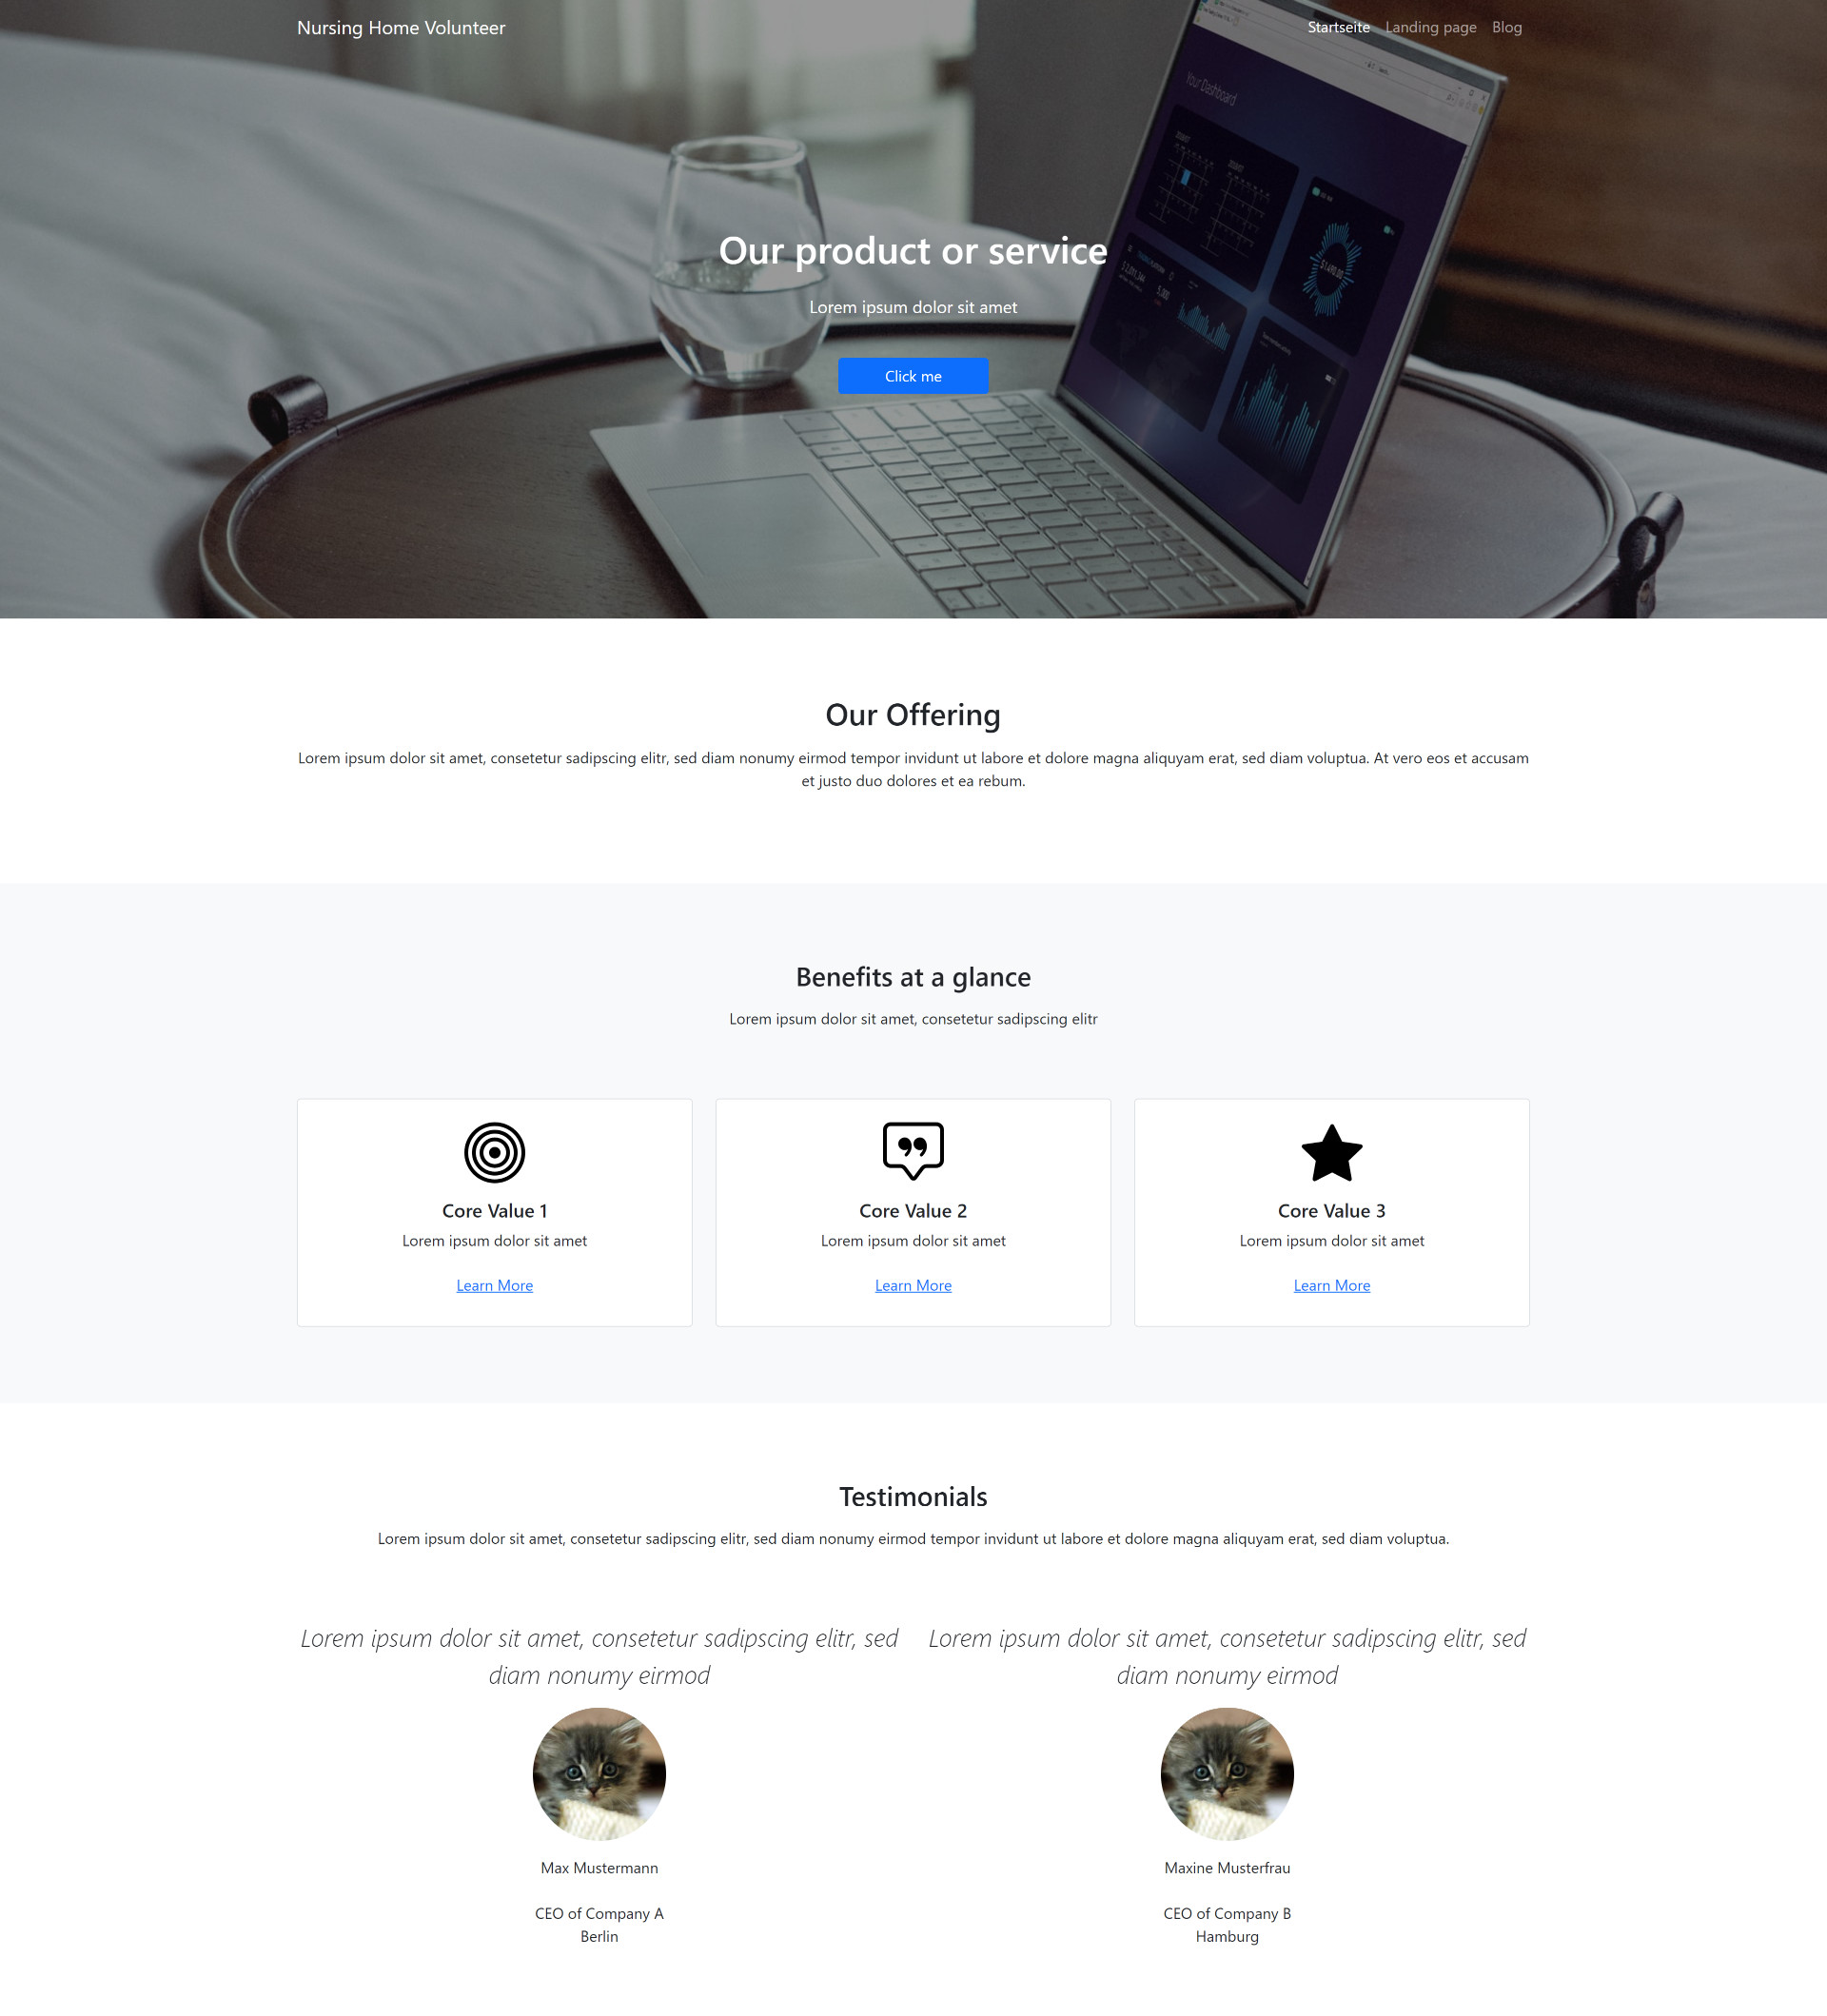
\includegraphics[width=0.9\textwidth]{images/frontend-homepage-1.jpg}}
  \centering
  \caption[Startseite des Frontends Teil 1]{Startseite des Frontends Teil 1}
  \label{fig:frontend-homepage-1}
\end{figure}

\begin{figure}[H]
  \setlength{\fboxsep}{0pt}
  \setlength{\fboxrule}{0.5pt}
  \fbox{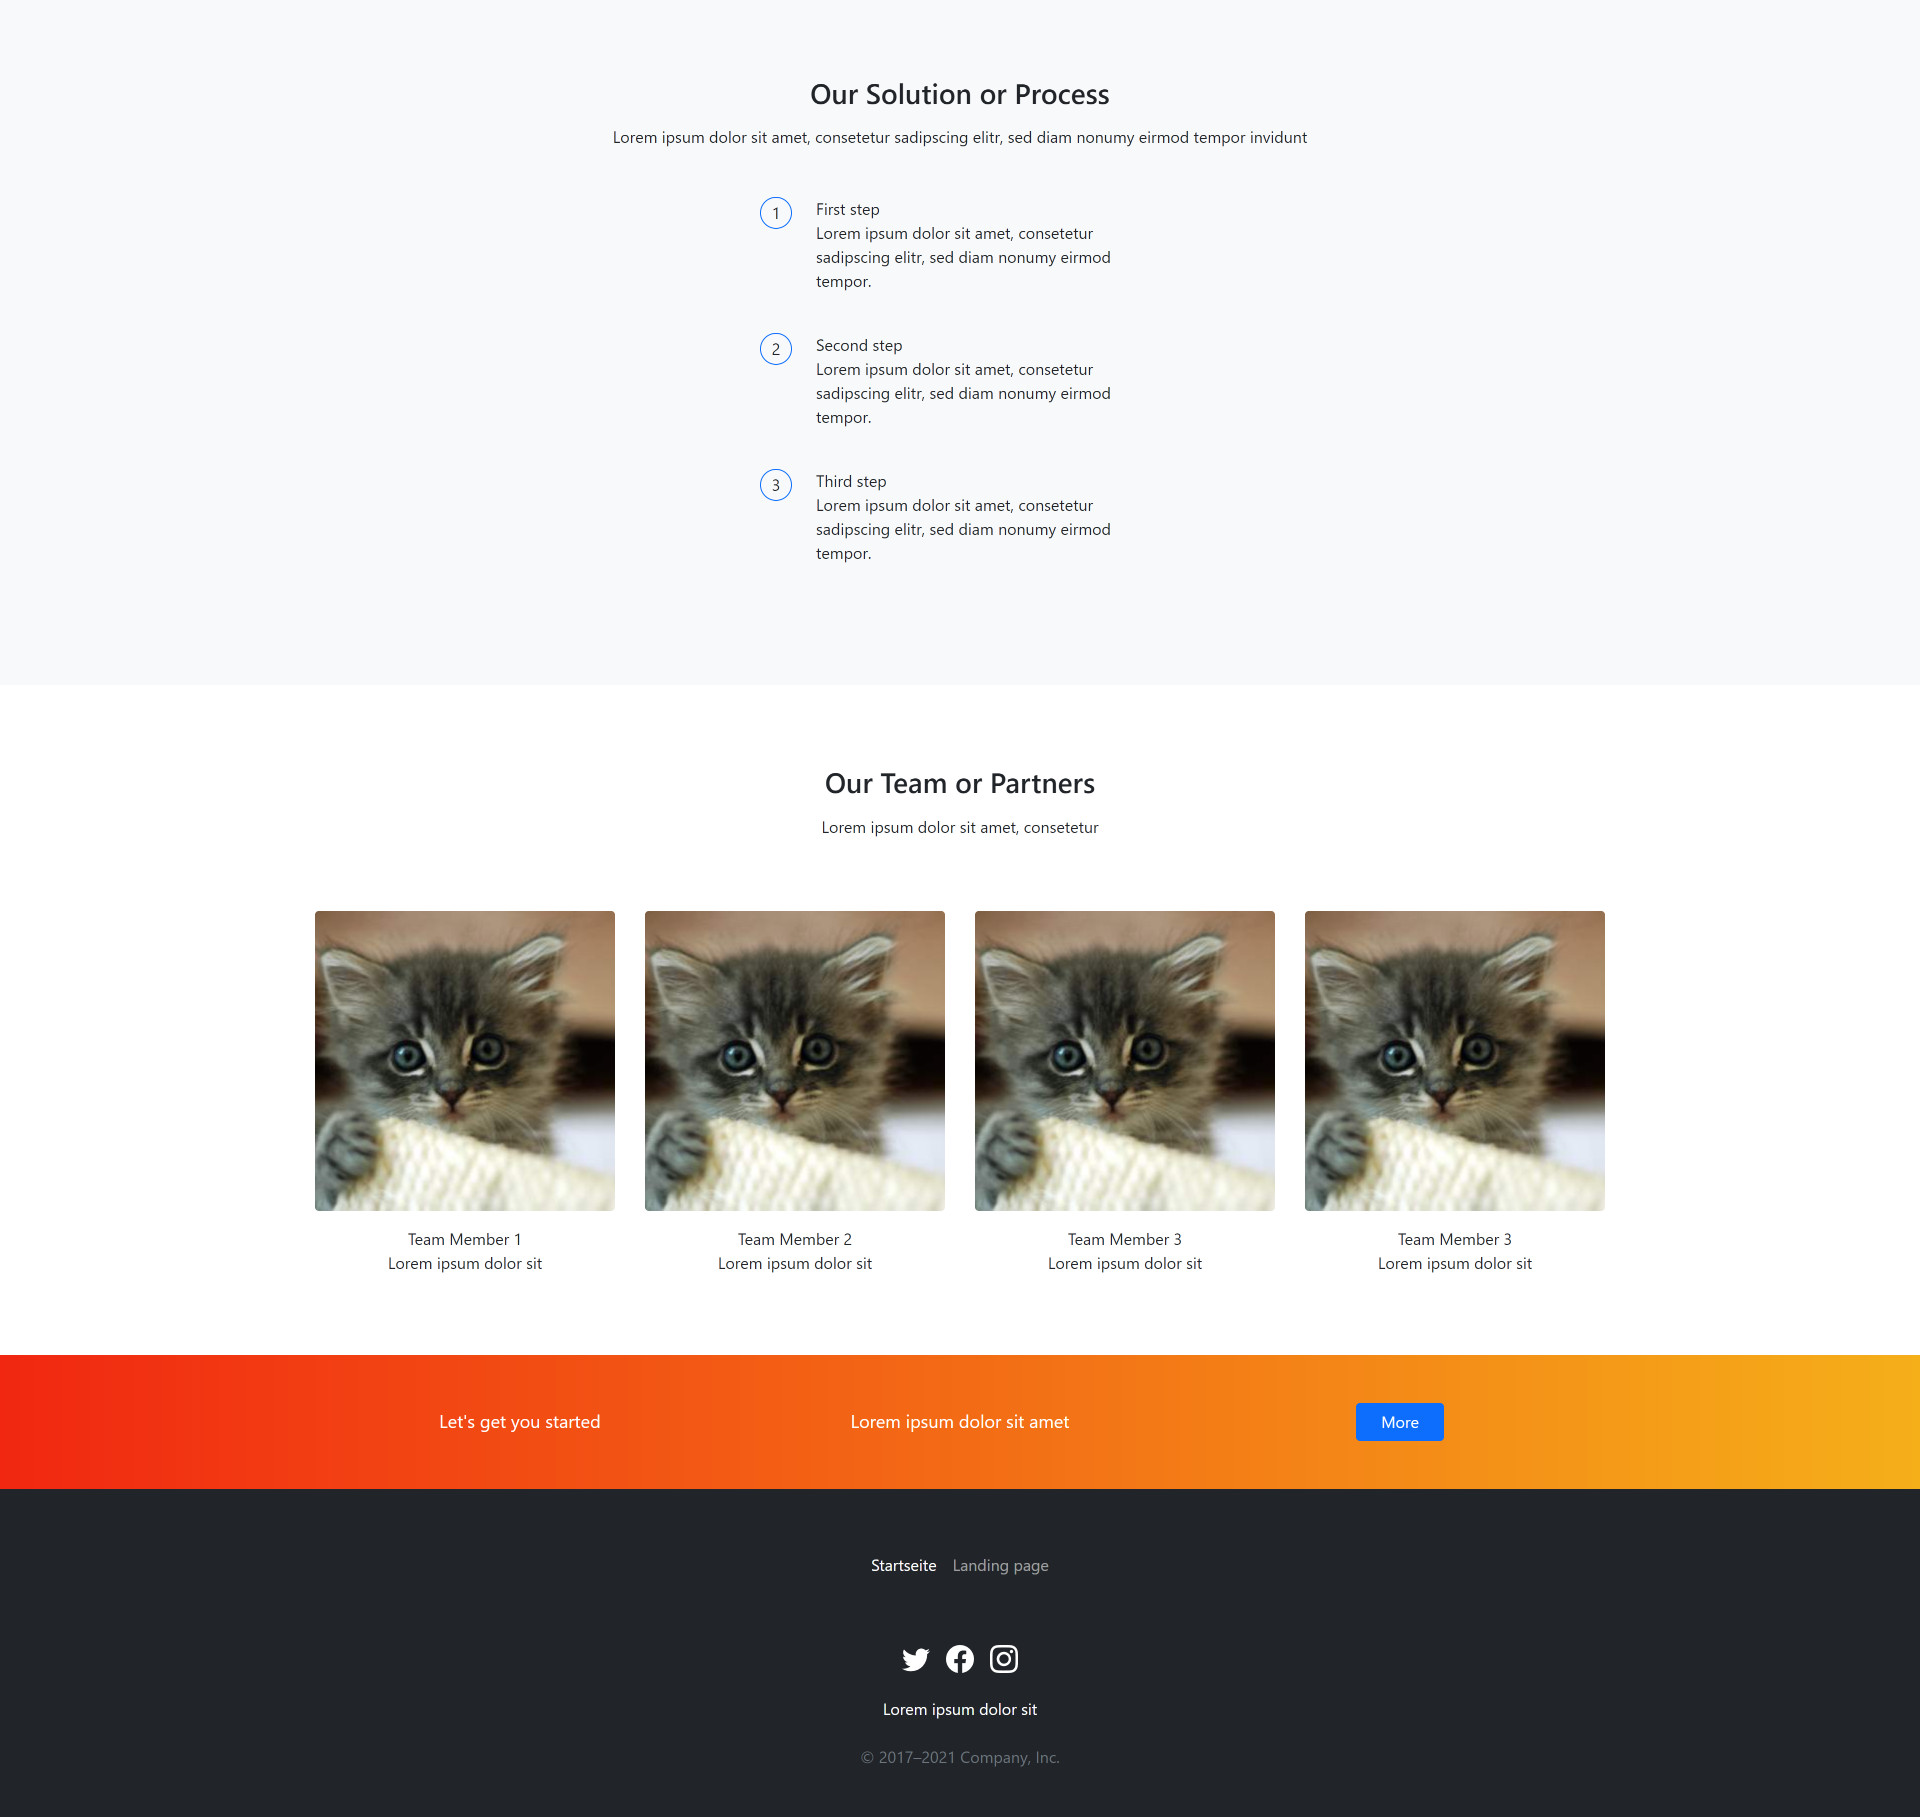
\includegraphics[width=0.9\textwidth]{images/frontend-homepage-2.jpg}}
  \centering
  \caption[Startseite des Frontends Teil 2]{Startseite des Frontends Teil 2}
  \label{fig:frontend-homepage-2}
\end{figure}

%
% Frontend - Landing page
%
\subsection{Landing page}

Die zweite Seite des Frontends ist die sogenannte landing page (siehe Abbildung \ref{fig:frontend-landing-page-1} und \ref{fig:frontend-landing-page-2}), die über die Route \lstinline{/landing-page} erreichbar ist. Diese Seite soll kurz und knapp die wichtigsten Informationen über das Angebot der Pflegeeinrichtung darstellen. Die landing page kann z.B. an Interessierte weitergeleitet werden, um diesen einen vollständigen und kompakten Überblick über alle Angebote zu geben. Alternativ kann diese Seite als Austausch für die Startseite verwendet werden, sollte dieser Wunsch seitens der Pflegeeinrichtung bestehen.

Hervorzuheben ist der interaktive Kopfbereich der Seite, indem der Besucher durch drei verschiedene Ansichten wechseln kann. In Abbildung \ref{fig:frontend-landing-page-1} ist der Hintergrund zwar lediglich grau, jedoch kann für jede Ansicht ein individuelles Hintergrundbild eingefügt werden, um die Seite ansprechender zu gestalten.

\begin{figure}[H]
  \setlength{\fboxsep}{0pt}
  \setlength{\fboxrule}{0.5pt}
  \fbox{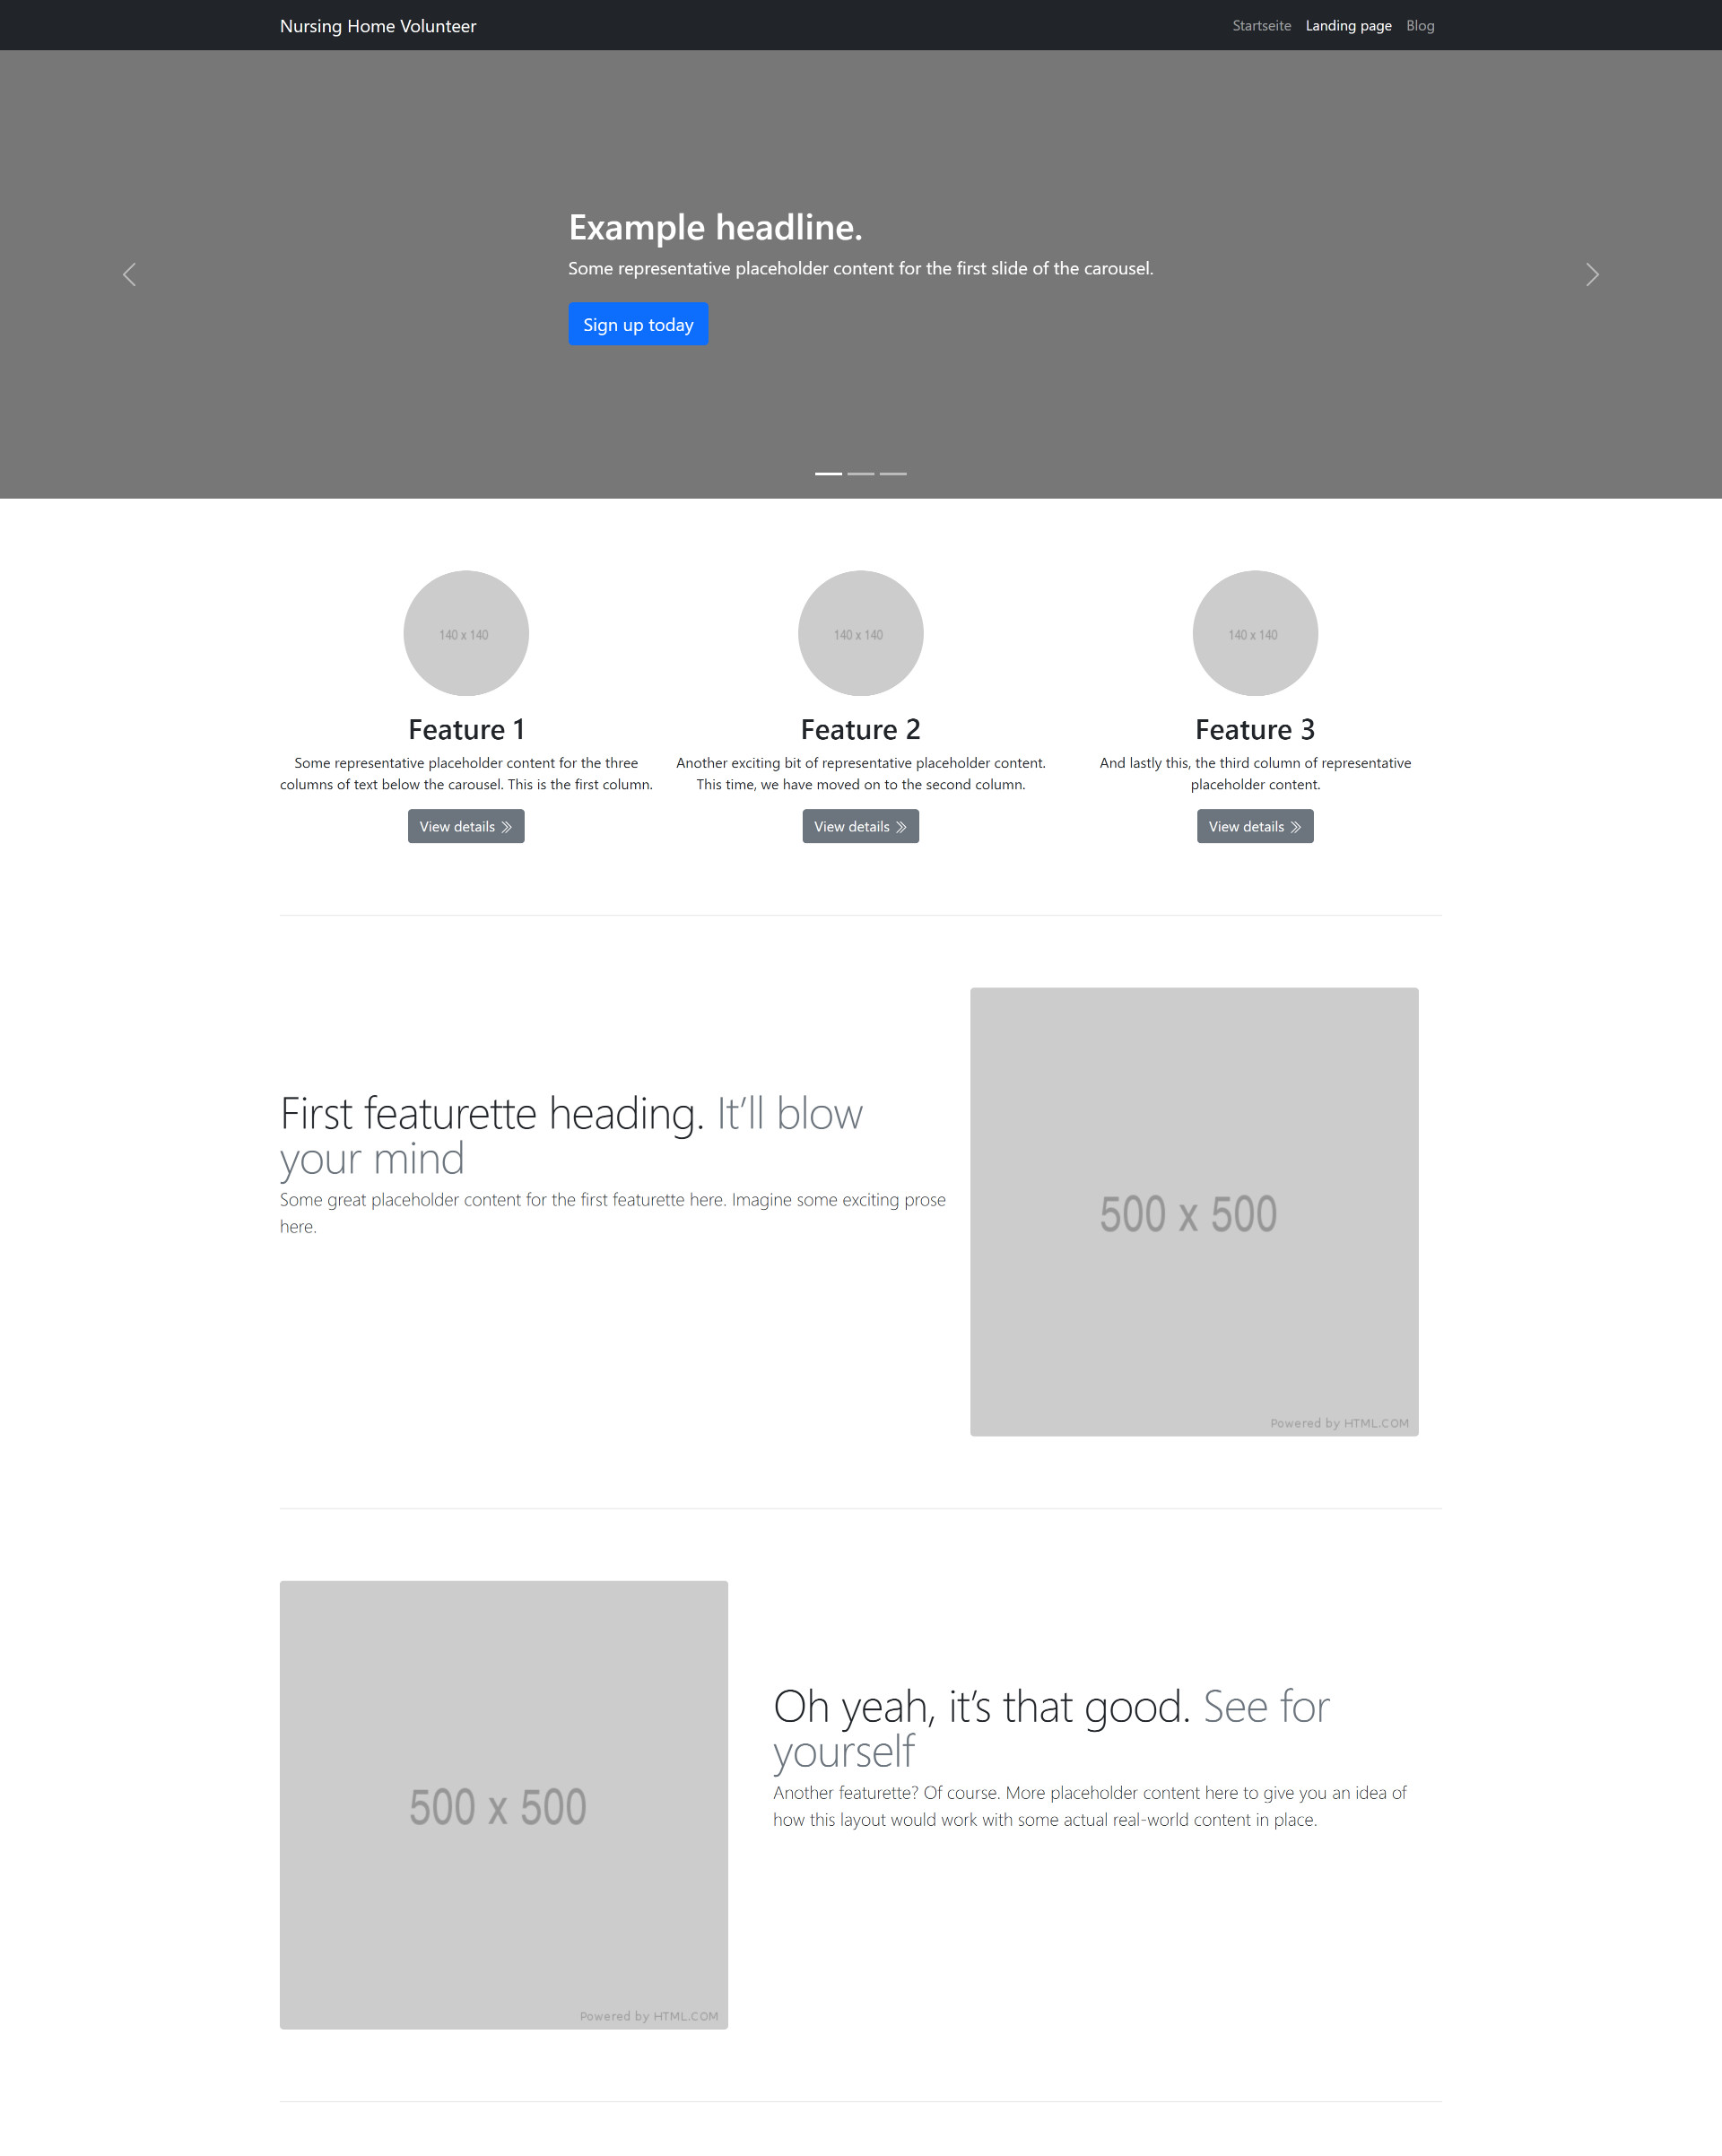
\includegraphics[width=0.85\textwidth]{images/frontend-landing-page-1.jpg}}
  \centering
  \caption[Landing page des Frontends Teil 1]{Landing page des Frontends Teil 1}
  \label{fig:frontend-landing-page-1}
\end{figure}

\begin{figure}[H]
  \setlength{\fboxsep}{0pt}
  \setlength{\fboxrule}{0.5pt}
  \fbox{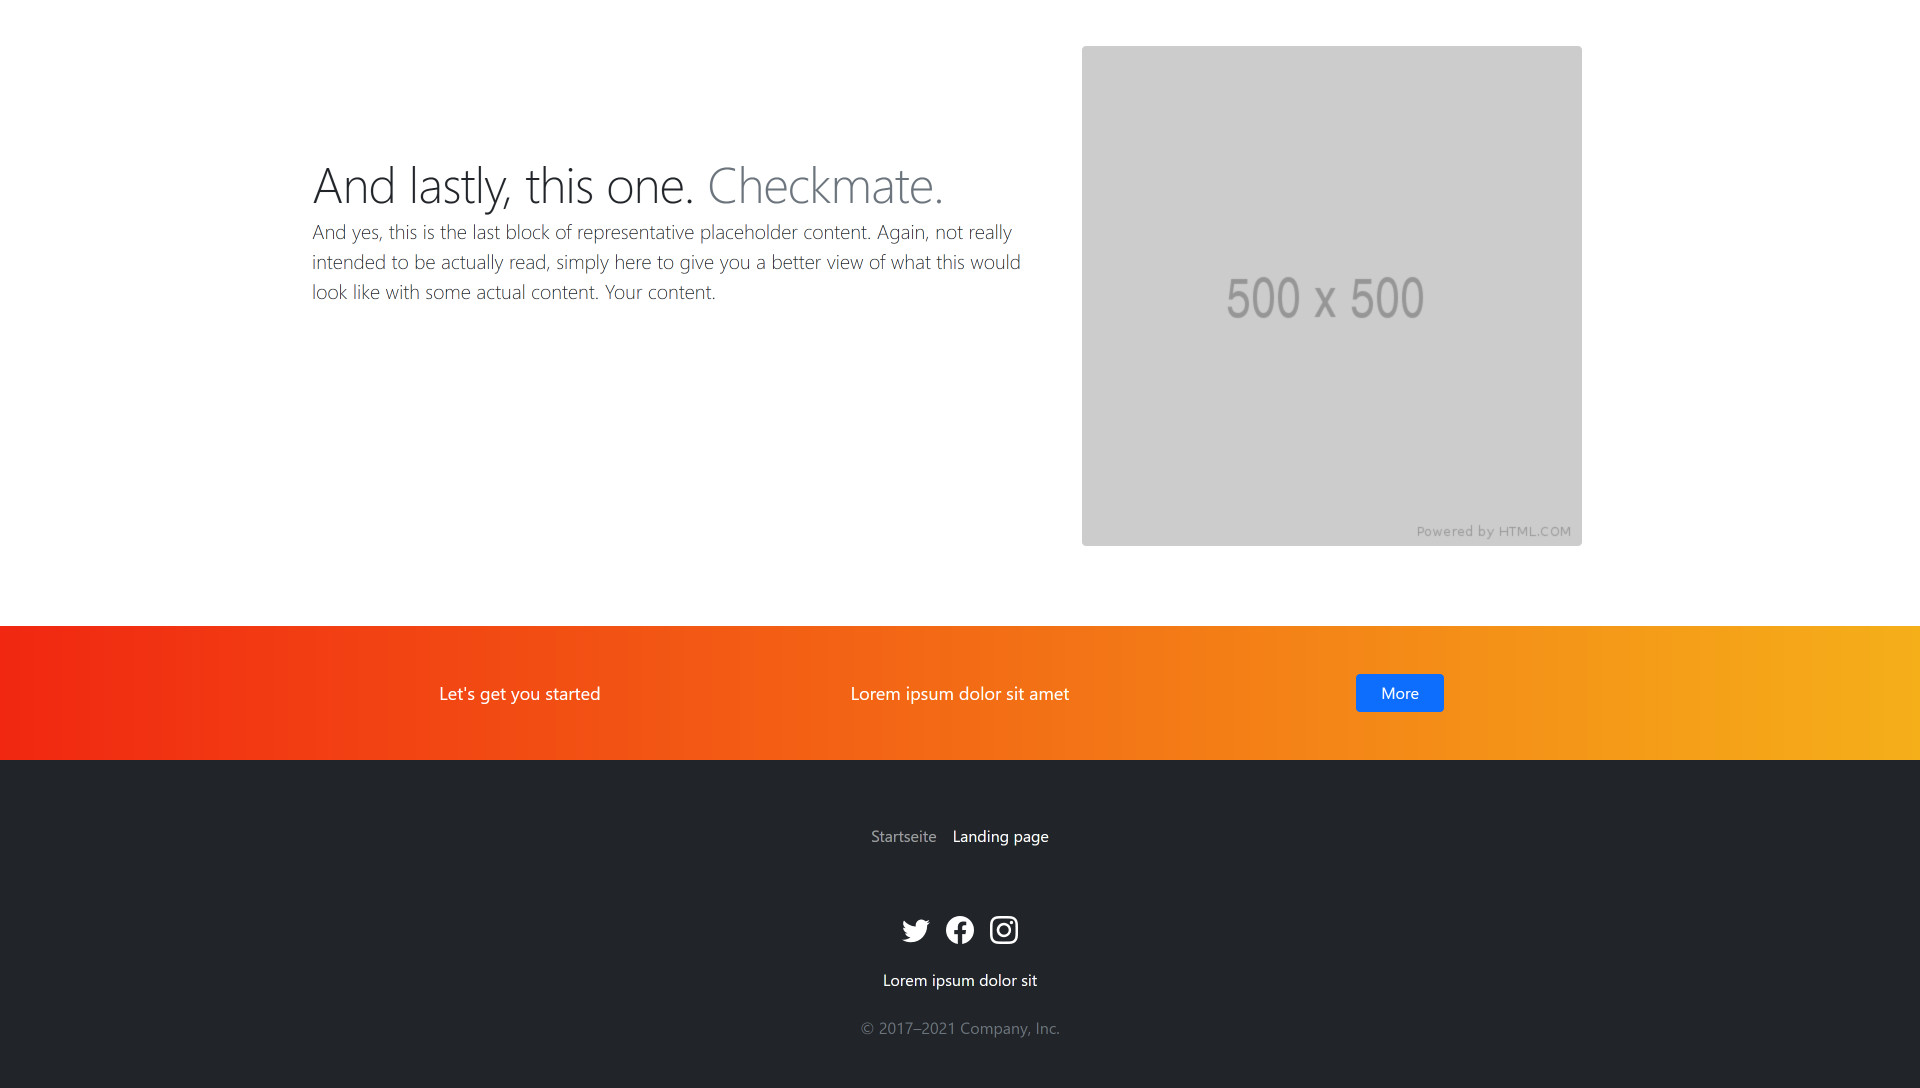
\includegraphics[width=0.9\textwidth]{images/frontend-landing-page-2.jpg}}
  \centering
  \caption[Landing page des Frontends Teil 2]{Landing page des Frontends Teil 2}
  \label{fig:frontend-landing-page-2}
\end{figure}

%
% Frontend - Blog
%
\subsection{Blog}

Der Blog ist die zentrale Stelle für die Ansicht aller Beiträge der Pflegeeinrichtung und ist über die Route \lstinline{/blog} erreichbar. Dabei werden alle verfügbaren Blogbeiträge vom Backend abgerufen und eine Vorschau dieser angezeigt. Ein Klick auf das Bild oder auf die \glqq Weiterlesen\grqq{}-Schaltfläche führt auf die Detailseite des Blogbeitrags.

Links neben den Blogbeiträgen befindet sich ein Platzhalter für Filtermöglichkeiten. Zum aktuellen Entwicklungsstand der Studienarbeit sind die Anforderungen für die Filter seitens der Pflegeeinrichtung noch nicht bekannt. Daher sind diese nicht implementiert.

\begin{figure}[H]
  \setlength{\fboxsep}{0pt}
  \setlength{\fboxrule}{0.5pt}
  \fbox{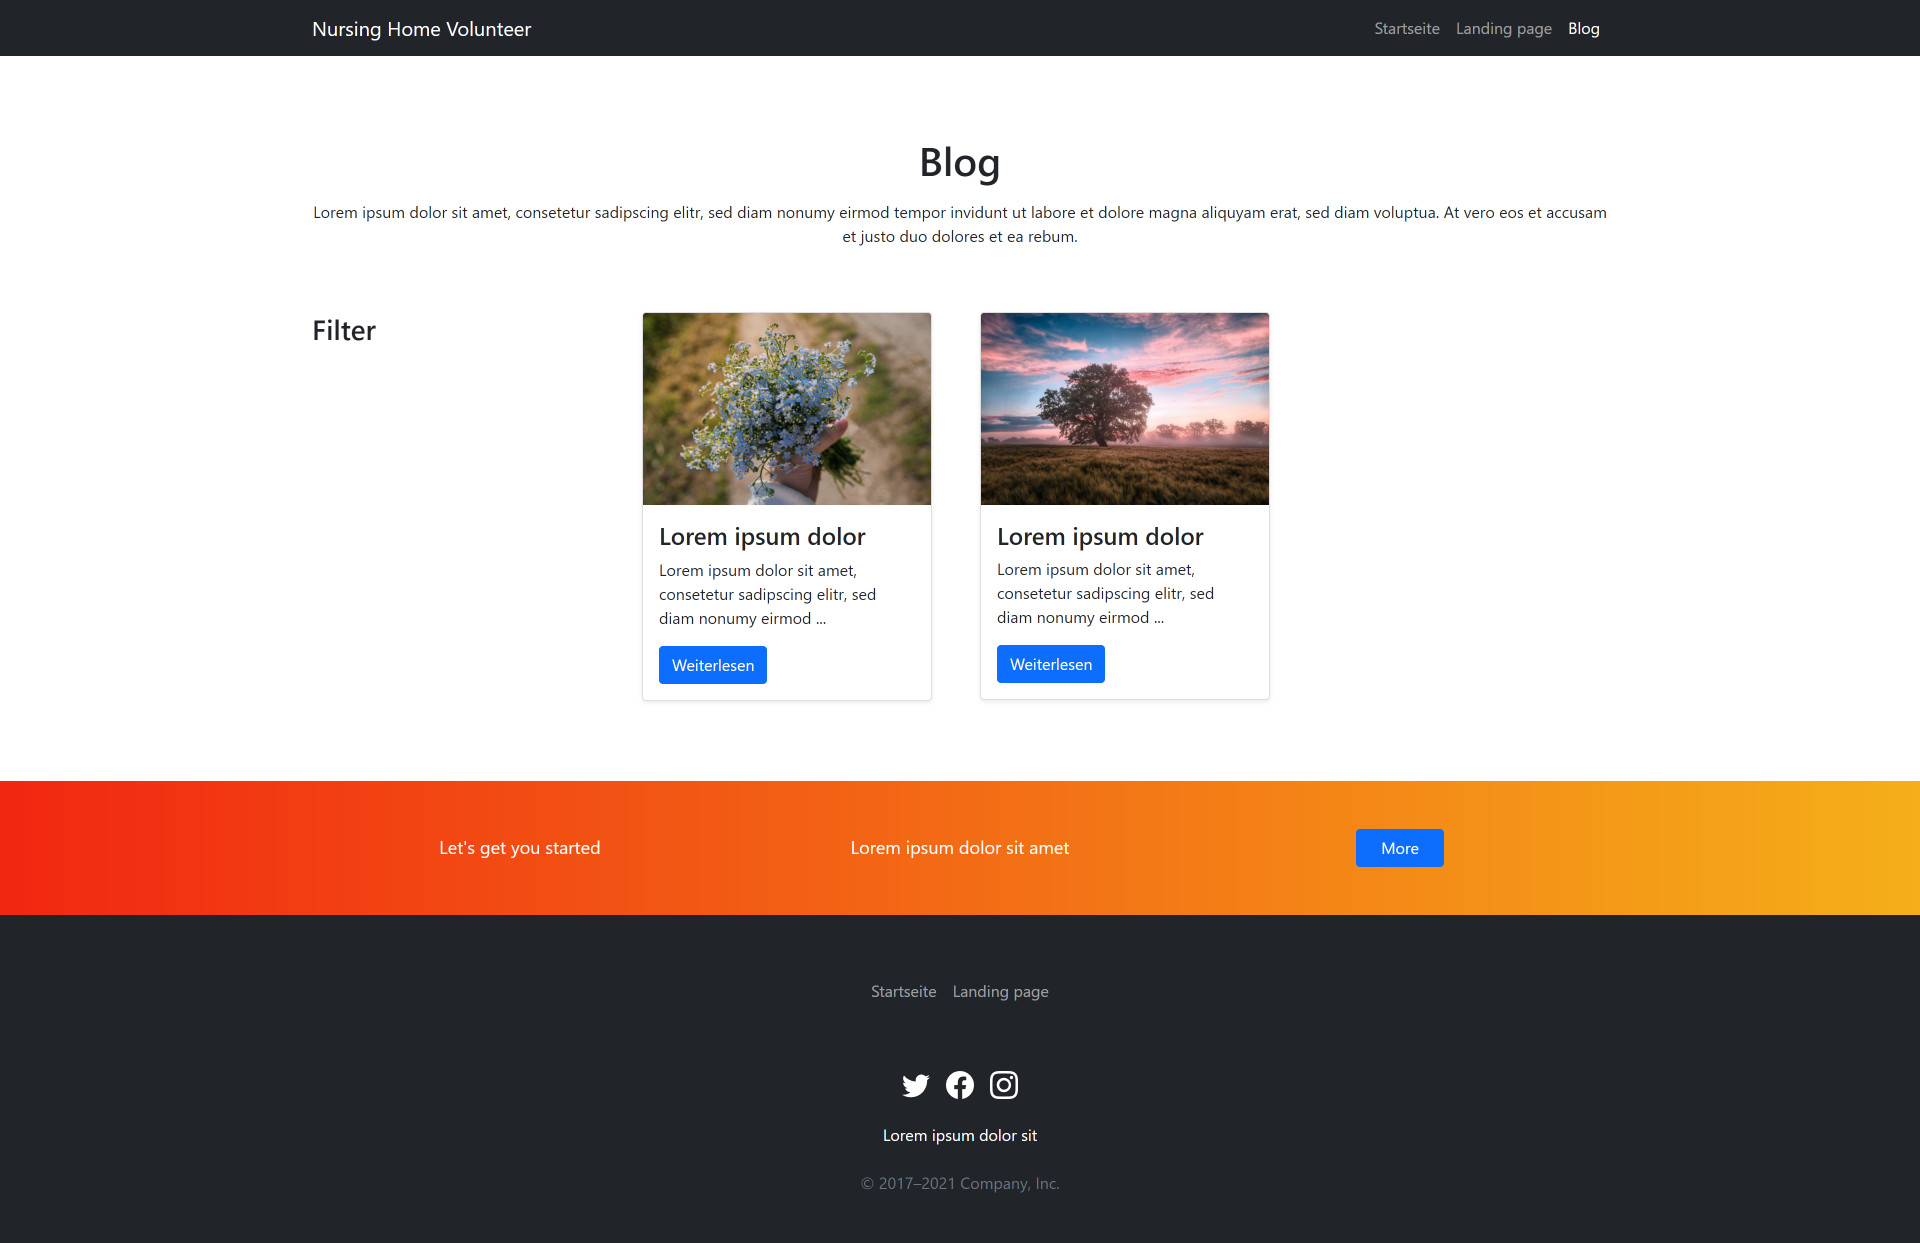
\includegraphics[width=0.9\textwidth]{images/frontend-blog.jpg}}
  \centering
  \caption[Blog des Frontends]{Blog des Frontends}
  \label{fig:frontend-blog}
\end{figure}

%
% Frontend - Blogbeitrag
%
\subsection{Blogbeitrag}

Nach dem Öffnen eines Beitrags im Blog oder durch manuellen Aufruf der URL, gelangt der Besucher auf die Detailseite für einen Blogbeitrag (siehe Abbildung \ref{fig:frontend-blogbeitrag}). Jeder Beitrag ist über die Route \lstinline{/blog/<id>} erreichbar, wobei \lstinline{<id>} durch die eindeutige ID des Beitrags ersetzt werden muss. Beim Aufruf der Seite wird der Blogbeitrag vom Backend abgerufen, falls dieser nicht bereits geladen wurde.

Ein Blogbeitrag besteht aus insgesamt vier Komponenten: Titel, Bild (optional), Beschreibung und beliebig vielen Medienbereichen.

Die Medienbereiche sind, wie in Abbildung \ref{fig:frontend-blogbeitrag} zu sehen, voneinander getrennte Abschnitte, die mindestens eine Beschreibung bzw. Text beinhalten. Der Titel sowie das Medium sind optional. Diese Bereiche können dazu verwendet werden, um den Blogbeitrag inhaltlich zu gliedern sowie mit weiteren Medien zu erweitern. Mögliche Medientypen sind Bilder, Videos, Audiodateien sowie sonstige Dateien (PDFs, Textdateien etc.).

\begin{figure}[H]
  \setlength{\fboxsep}{0pt}
  \setlength{\fboxrule}{0.5pt}
  \fbox{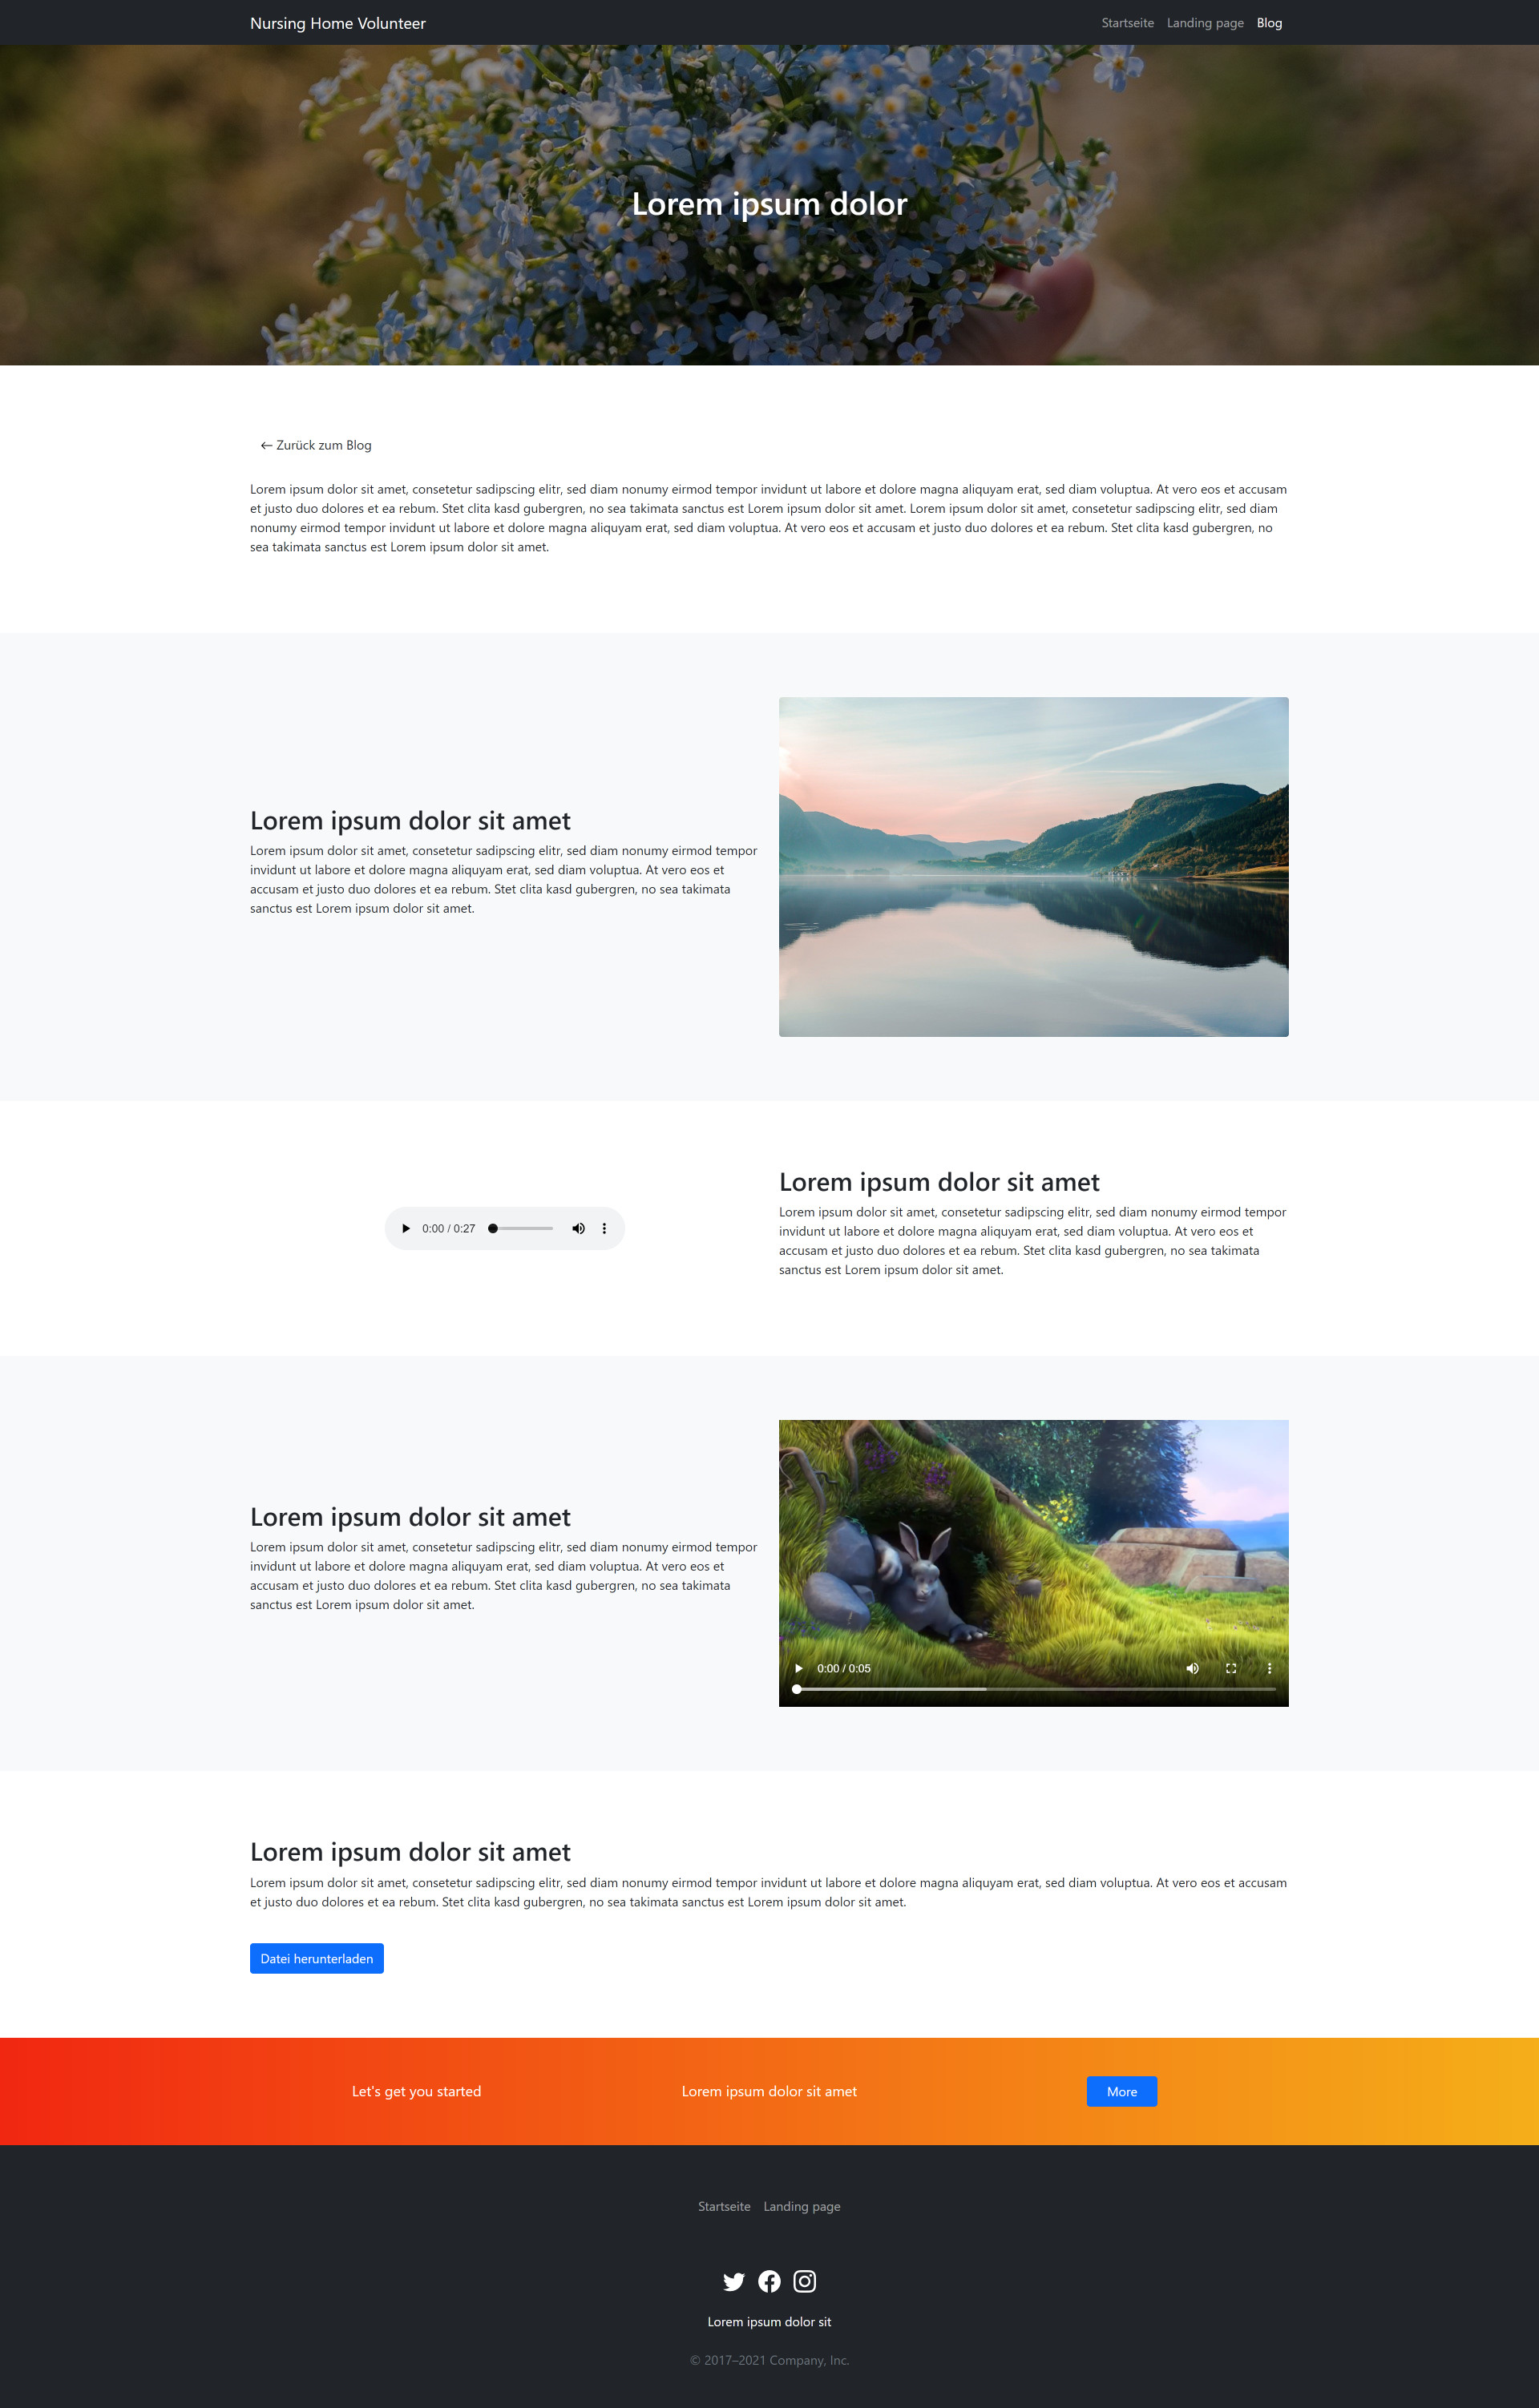
\includegraphics[width=0.85\textwidth]{images/frontend-blogbeitrag.jpg}}
  \centering
  \caption[Blogbeitrag des Frontends]{Blogbeitrag des Frontends}
  \label{fig:frontend-blogbeitrag}
\end{figure}

%
% Frontend - Code-Struktur
%
\subsection{Code-Struktur}

Tabelle \ref{tbl:frontend-struktur} zeigt die hierarchische Code-Struktur des Frontends sowie die Funktionen der wesentlichen Verzeichnisse und Dateien.

\begin{table}[ht!]
  \begin{center}
    \resizebox{0.9\textwidth}{!}{
      \begin{tabular}{|l|l|}
        \hline
        Ordner / Datei  & Beschreibung                                                         \\ \hline
        assets          & Bilder/Dateien, die im Frontend verwendet werden (außer Favicons)    \\ \hline
        axios           & REST-Client zur Interaktion mit dem Backend                          \\ \hline
        components      & Vue-Komponenten (\acp{SFC})                                          \\ \hline
        \quad bootstrap & Komponenten, die mithilfe von Bootstrap erstellt wurden              \\ \hline
        \quad layouts   & Layout- bzw. Struktur-Komponenten (z.B. Header, Hauptinhalt, Footer) \\ \hline
        config          & Statische Konfiguration des Frontends (z.B. URL des Backends)        \\ \hline
        router          & Vue Router zur Navigation zwischen den Seiten                        \\ \hline
        store           & Globaler Zustand / Daten (z.B. Blogbeiträge)                         \\ \hline
        styles          & Globales CSS / Sass                                                  \\ \hline
        types           & TypeScript Typ-Definitionen                                          \\ \hline
        utils           & Globale (wiederverwendbare) Funktionen                               \\ \hline
        views           & Vue-Komponenten für die Seiten                                       \\ \hline
        App.vue         & App-Komponente (Eintrittspunkt / Hauptkomponente des Frontends)      \\ \hline

      \end{tabular}
    }
    \caption[Beschreibung der wesentlichen Verzeichnisse und Dateien des Frontends]{Beschreibung der wesentlichen Verzeichnisse und Dateien des Frontends}
    \label{tbl:frontend-struktur}
  \end{center}
\end{table}

%
% Frontend - Lokale Entwicklung
%
\subsection{Lokale Entwicklung}

Details zur lokalen Entwicklung des Frontends befinden sich in der Datei \glqq \lstinline{frontend/README.md}\grqq{}. Nachdem ein Kommandozeilen-Fenster geöffnet und der Pfad zu den Dateien des Frontends geöffnet wurde, muss zuerst durch den Befehl \glqq \lstinline{npm install}\grqq{} die Abhängigkeiten bzw. Pakete installiert werden, die das Frontend verwendet. Anschließend kann das Frontend durch \glqq \lstinline{npm run dev}\grqq{} für die Entwicklung gestartet werden, wodurch es unter der URL \glqq \lstinline{http://localhost:3000}\grqq{} zur Verfügung steht. Bei Änderungen am Code wird die Seite automatisch aktualisiert.

Um das Frontend für den Produktivbetrieb zu kompilieren, muss der Befehl \glqq \lstinline{npm run build}\grqq{} verwendet werden. Hierdurch wird ein \glqq \lstinline{dist}\grqq{}-Ordner erstellt, der die kompilierten statischen Dateien des Frontends beinhaltet.

\section{Backend}
\label{sec:struktur-backend}

\begin{figure}[H]
  \setlength{\fboxsep}{0pt}
  \setlength{\fboxrule}{0.5pt}
  \fbox{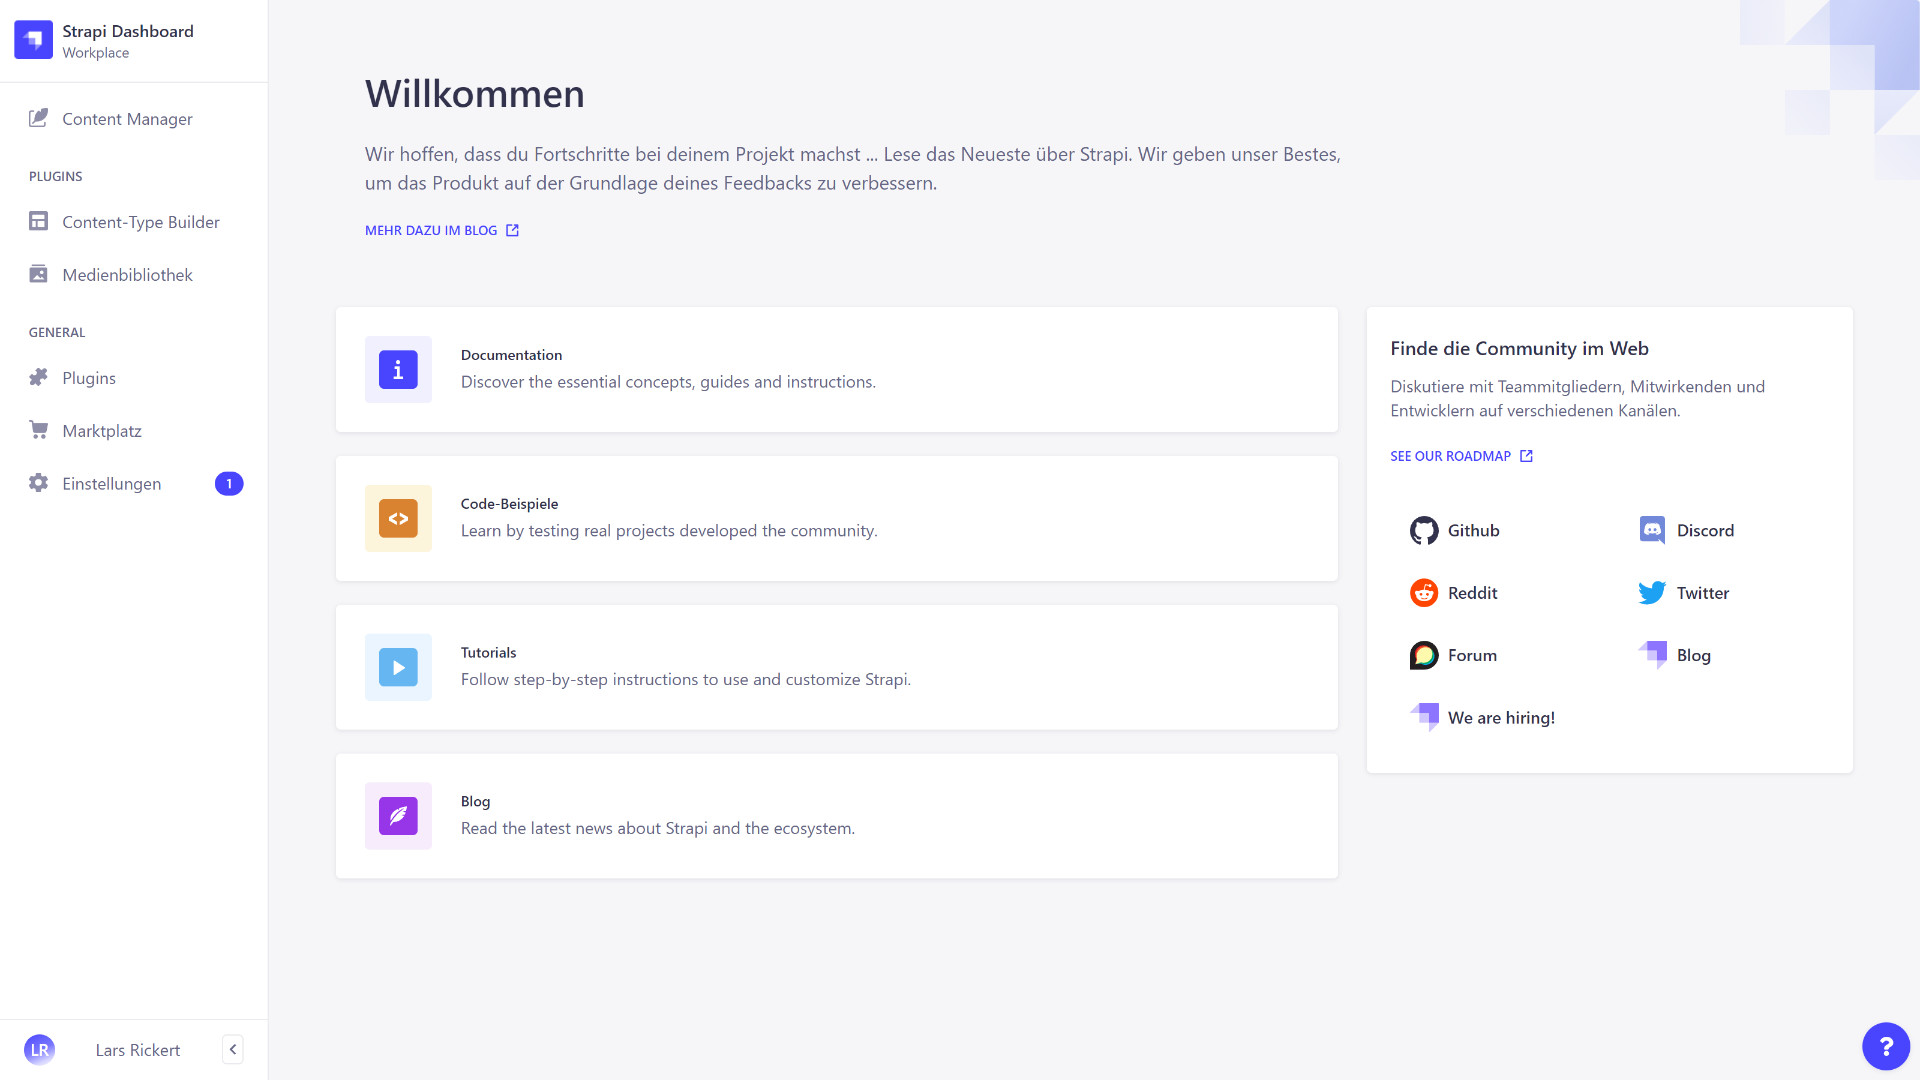
\includegraphics[width=0.9\textwidth]{images/backend-dashboard.jpg}}
  \centering
  \caption[Dashboard des Backends]{Dashboard des Backends}
  \label{fig:backend-dashboard}
\end{figure}

Abbildung \ref{fig:backend-dashboard} zeigt das Dashboard bzw. die Startseite des Backends, das über die Route \lstinline{/admin} erreichbar ist. Unter dem Menüpunkt \glqq Content-Type Builder\grqq{} können über die Benutzeroberfläche Inhaltstypen angelegt werden, die dann über die API zugänglich sind (siehe Abbildung \ref{fig:backend-content-type-builder}). Im Rahmen dieser Studienarbeit wurde ein Inhaltstype \glqq Blog Post\grqq{} angelegt, der das Erstellen von Blogbeiträgen ermöglicht. Die Inhaltstypen können lediglich während der Entwicklung geändert werden. Im Produktivbetrieb ist dies nicht mehr möglich.

Die konkreten Inhalte für den Inhaltstyp, d.h. die Blogbeiträge können anschließend unter dem Menüpunkt \glqq Content Manager\grqq{} verwaltet werden.

\begin{figure}[H]
  \setlength{\fboxsep}{0pt}
  \setlength{\fboxrule}{0.5pt}
  \fbox{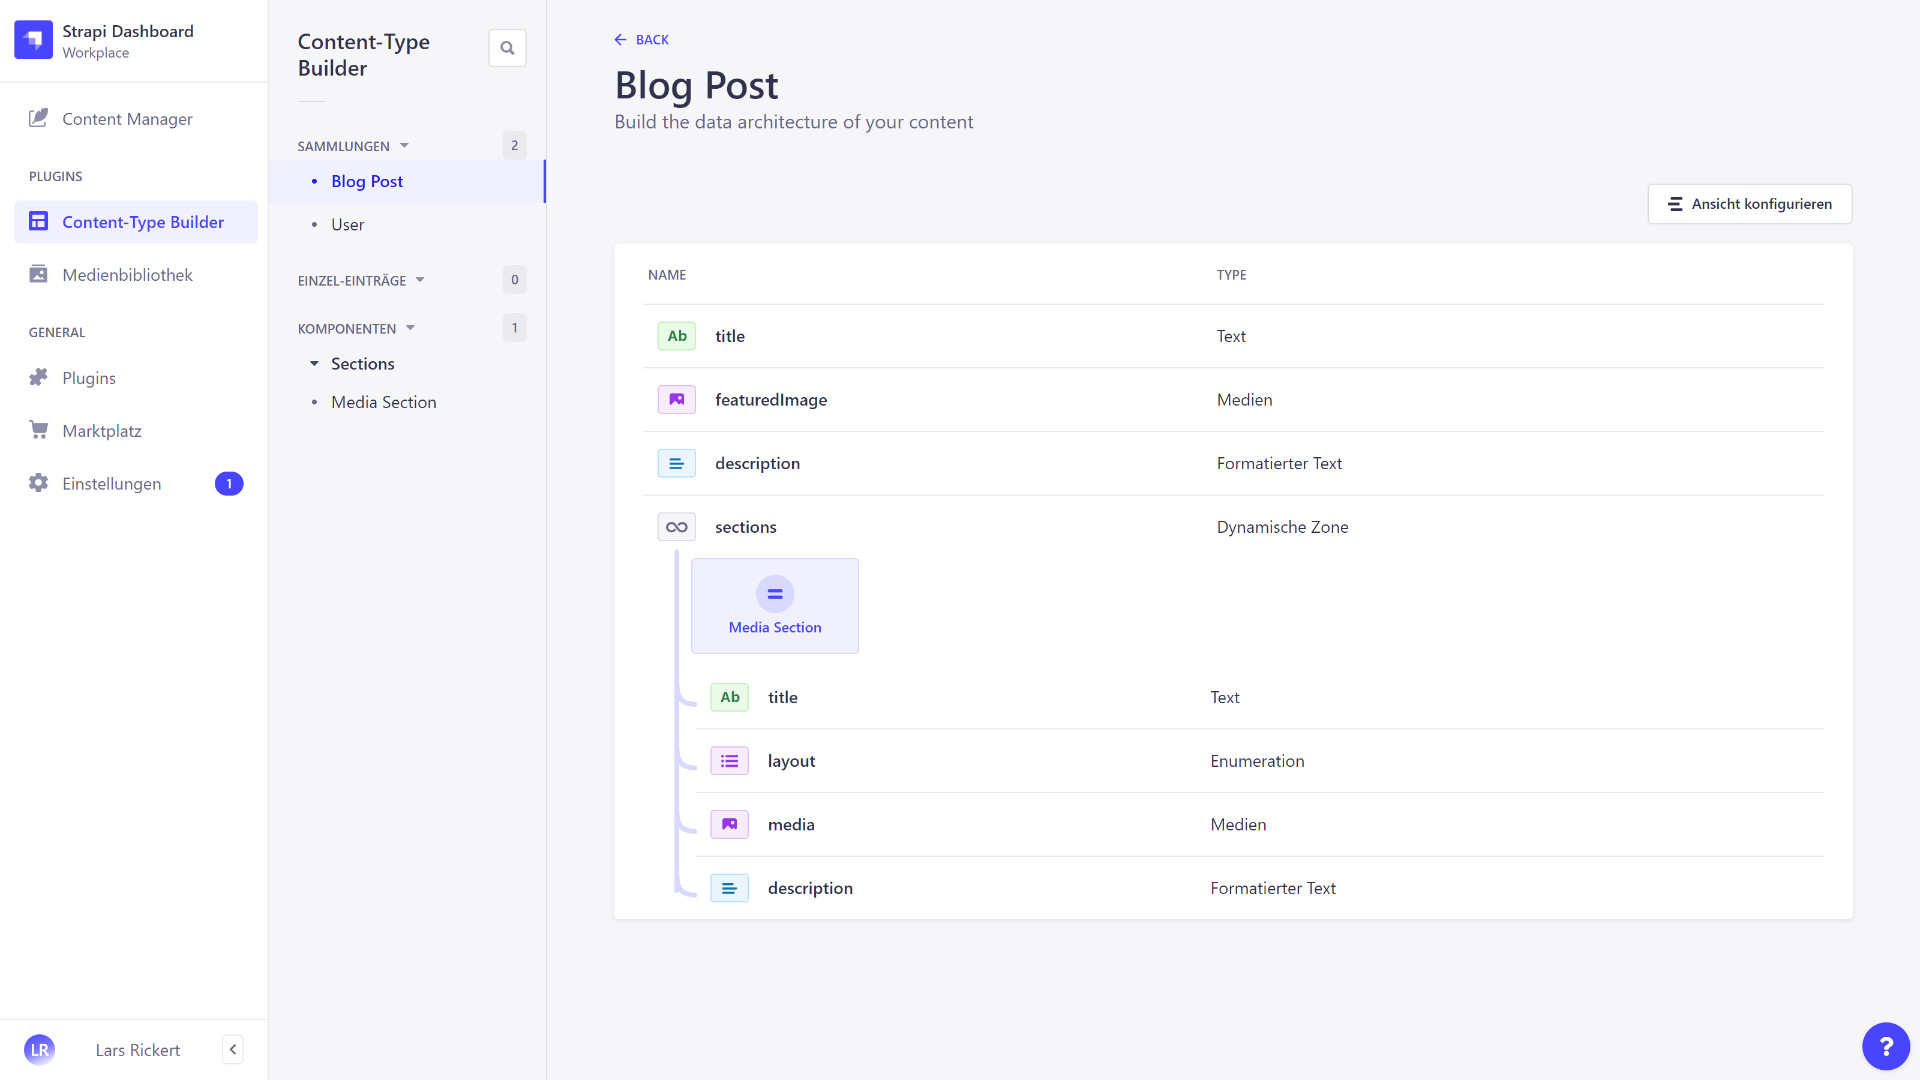
\includegraphics[width=0.9\textwidth]{images/backend-content-type-builder.jpg}}
  \centering
  \caption[Inhaltstyp für die Blogbeiträge]{Inhaltstyp für die Blogbeiträge}
  \label{fig:backend-content-type-builder}
\end{figure}

\textbf{Lokale Entwicklung} \\
So wie bei der lokalen Entwicklung des Frontends muss zuerst ein Kommandozeilen-Fenster und darin der Pfad zu den Dateien des Backends geöffnet werden. Anschließend müssen ebenfalls die Abhängigkeiten bzw. Pakete, die das Backend verwendet mit \glqq \lstinline{npm install}\grqq{} installiert werden.

Für die lokale Entwicklung des Backends kann dieses mit \glqq \lstinline{npm run develop}\grqq{} gestartet werden. Für den Produktivbetrieb muss es zuerst mit \glqq \lstinline{npm run build}\grqq{} kompiliert und danach mit \glqq \lstinline{npm start}\grqq{} gestartet werden.

Für weitere Informationen über Strapi sei für Interessierte auf \cite{Strapi} verwiesen.
